\section{Problem Description}\label{sec:prob_descr}
A cantilevered unbalanced helicopter needs to be balanced using optimizing control.
The complete model of the helicopter is outlined in equation \ref{eq:model}.
\begin{subequations}\label{eq:model}
	\begin{align}
		\ddot{e} + K_{3} K_{ed} \dot{e} + K_{3} K_{ep} e = K_{3} K_{ep} e_{c} \label{eq:model_se_elev} \\
		\ddot{p} + K_{1} K_{pd} \dot{p} + K_{1} K_{pp} p = K_{1} K_{pp} p_{c} \label{eq:model_se_pitch} \\
		\dot{\lambda} = r \label{eq:model_se_lambda} \\
		\dot{r} = -K_{2} p \label{eq:model_se_r}
	\end{align}
\end{subequations}

The specific exercises can be found in the appendix. The exercises are located in sections 10.2, 10.3, and 10.4 of appendix.

\subsection{Illustrations}
% If you decide to include an illustration, that's great. You can in general copy figures and illustrations from the textbook, the assignement text, or other places. However: ALWAYS CITE THE SOURCE\@. You can also draw your own (cite the source if it is heavily based on someone else's.). \Cref{fig:layers_openloop} was created quickly with Ipe (\url{http://ipe.otfried.org/}). Inkscape is a good alternative for more advanced illustrations. Some people prefer the Latex package TikZ (\url{http://texample.net/tikz/examples/}), but this takes a little effort to learn.
The following picture describes the lab setup.

% \begin{figure}[tp]
% 	\centering
% 	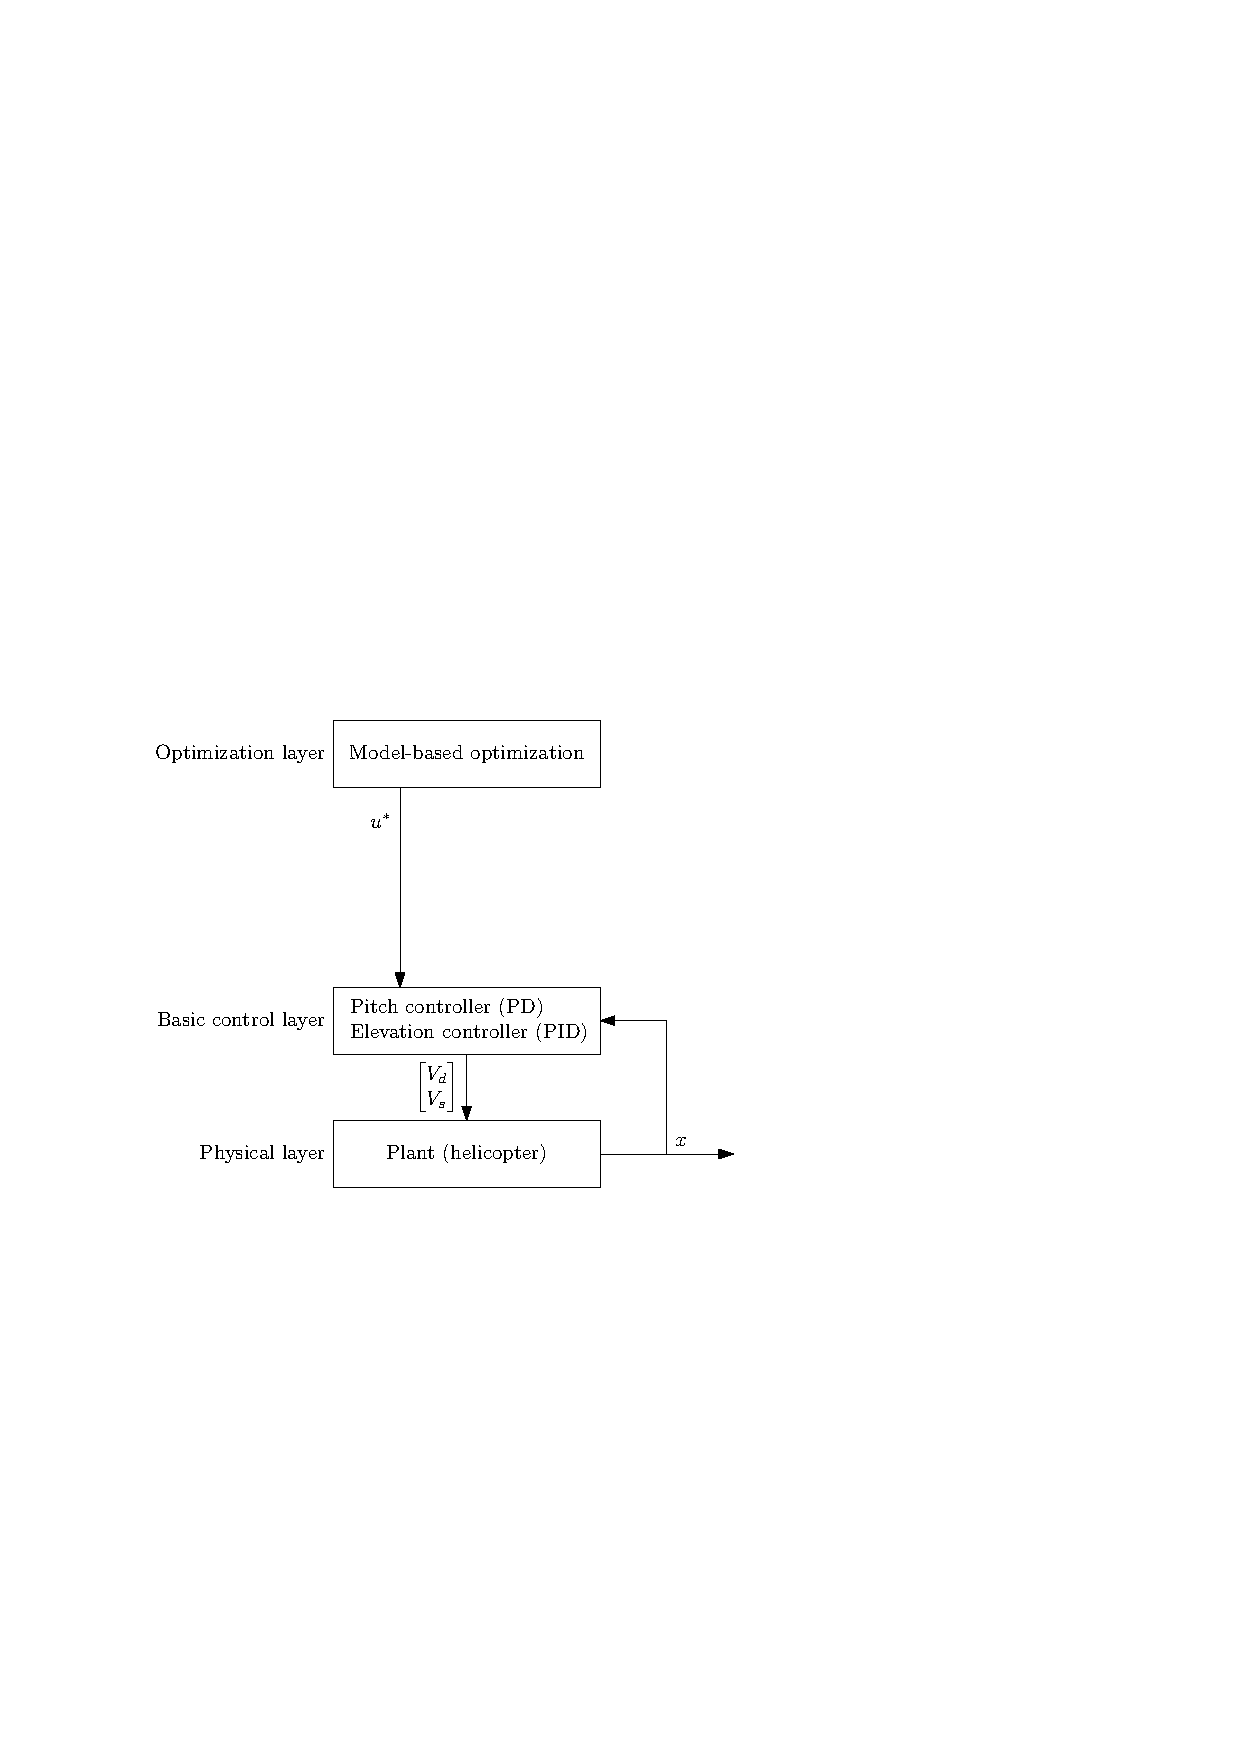
\includegraphics[width=1.00\textwidth]{figures/layers_openloop.pdf}
% 	\caption{A figure created with Ipe for TTK4135.}
% \label{fig:layers_openloop}
% \end{figure}
